% =====================================================================
%  Figure captions for the eight validation panels of
%  semantic-causal-propagation.tex. Included via \input from the main
%  manuscript's Numerical Validation section.
% =====================================================================

\begin{figure*}[!htbp]
    \centering
    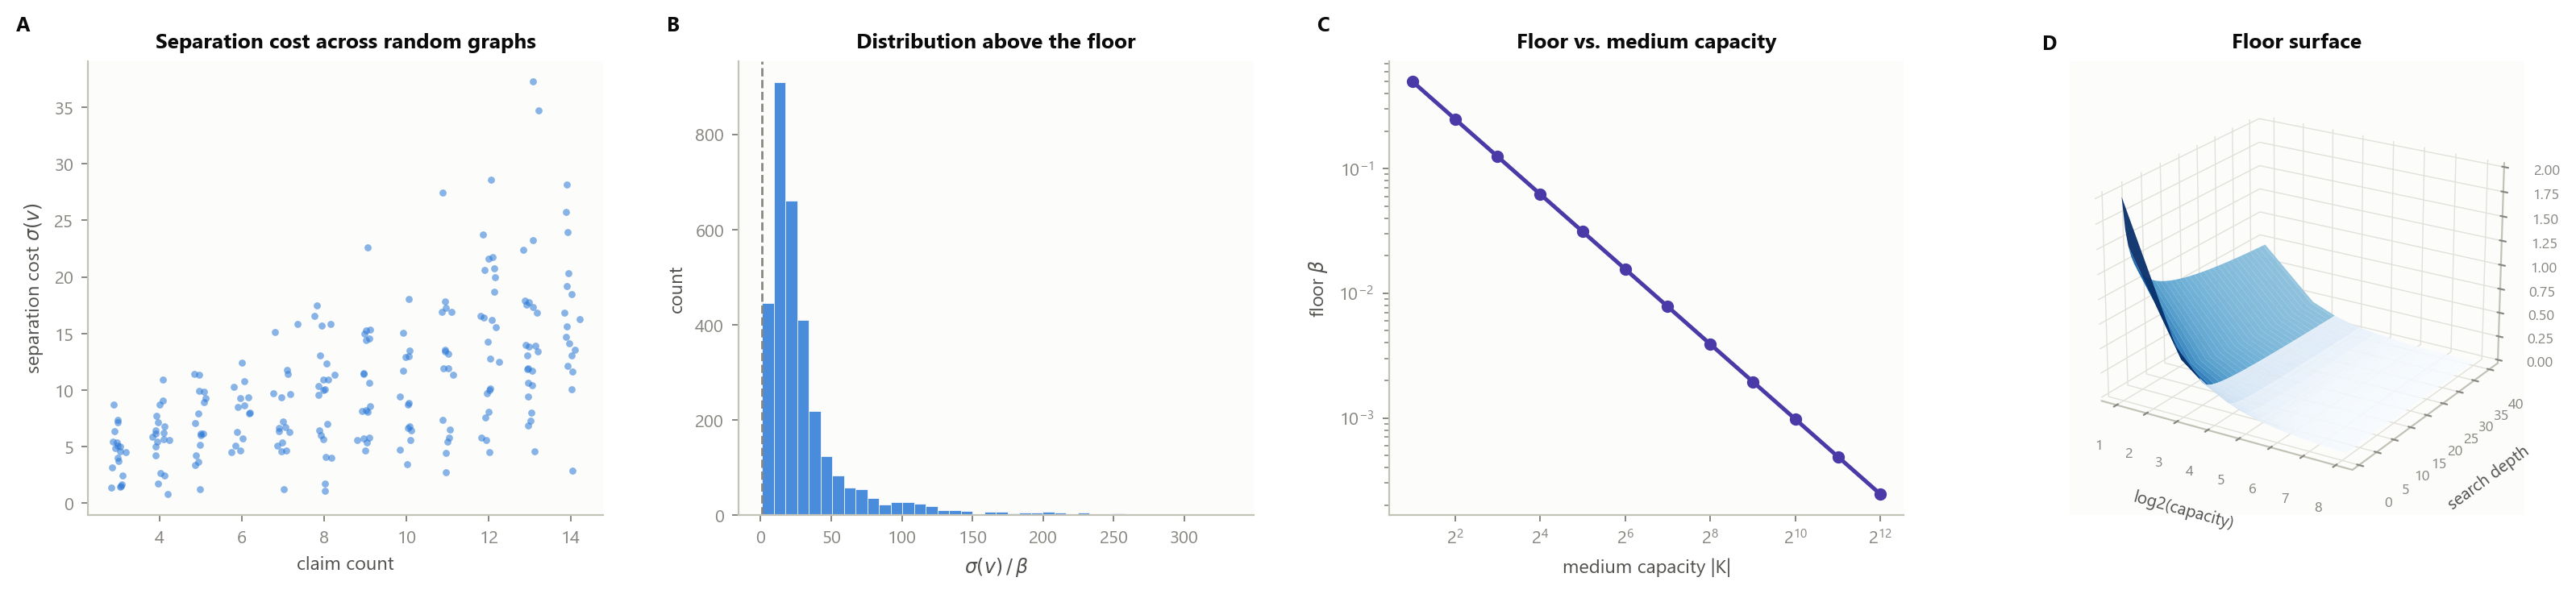
\includegraphics[width=\textwidth]{figures/panel_01_floor.png}
    \caption{\textbf{The Resolution Floor.}
    (\textbf{A})~Separation cost $\sigma(v)$ against claim count, one point
    per claim across $220$ random contact graphs of $3$--$14$ claims (steelblue).
    Cost rises with claim count but never falls below the graph's own floor
    $\beta$, the empirical content of Theorem~\ref{thm:floor}: no claim is
    individuated for free, regardless of how large the medium is.
    (\textbf{B})~Distribution of the ratio $\sigma(v)/\beta$ across $400$
    random graphs and all their claims; the dashed line marks $\sigma/\beta=1$.
    The histogram is supported entirely at and above the floor: no claim of
    any constructed instance is separated from the medium below the
    theorem's bound (Corollary~\ref{cor:no-sharp}).
    (\textbf{C})~Floor value against medium capacity $|K|$ on log-log axes,
    for twelve capacities $|K|\in\{2,4,\dots,4096\}$. The floor falls
    monotonically as capacity grows but remains strictly positive at every
    tested capacity, confirming that a larger medium narrows, but never
    closes, the resolution floor.
    (\textbf{D})~Three-dimensional surface of the floor over medium
    capacity (log scale) and search depth: the surface is bounded below by
    the inverse-capacity term and decays toward it as depth increases,
    never reaching zero. The floor is a property of the medium's finiteness,
    not of how long the search runs.}
    \label{fig:panel1-floor}
\end{figure*}

\begin{figure*}[!htbp]
    \centering
    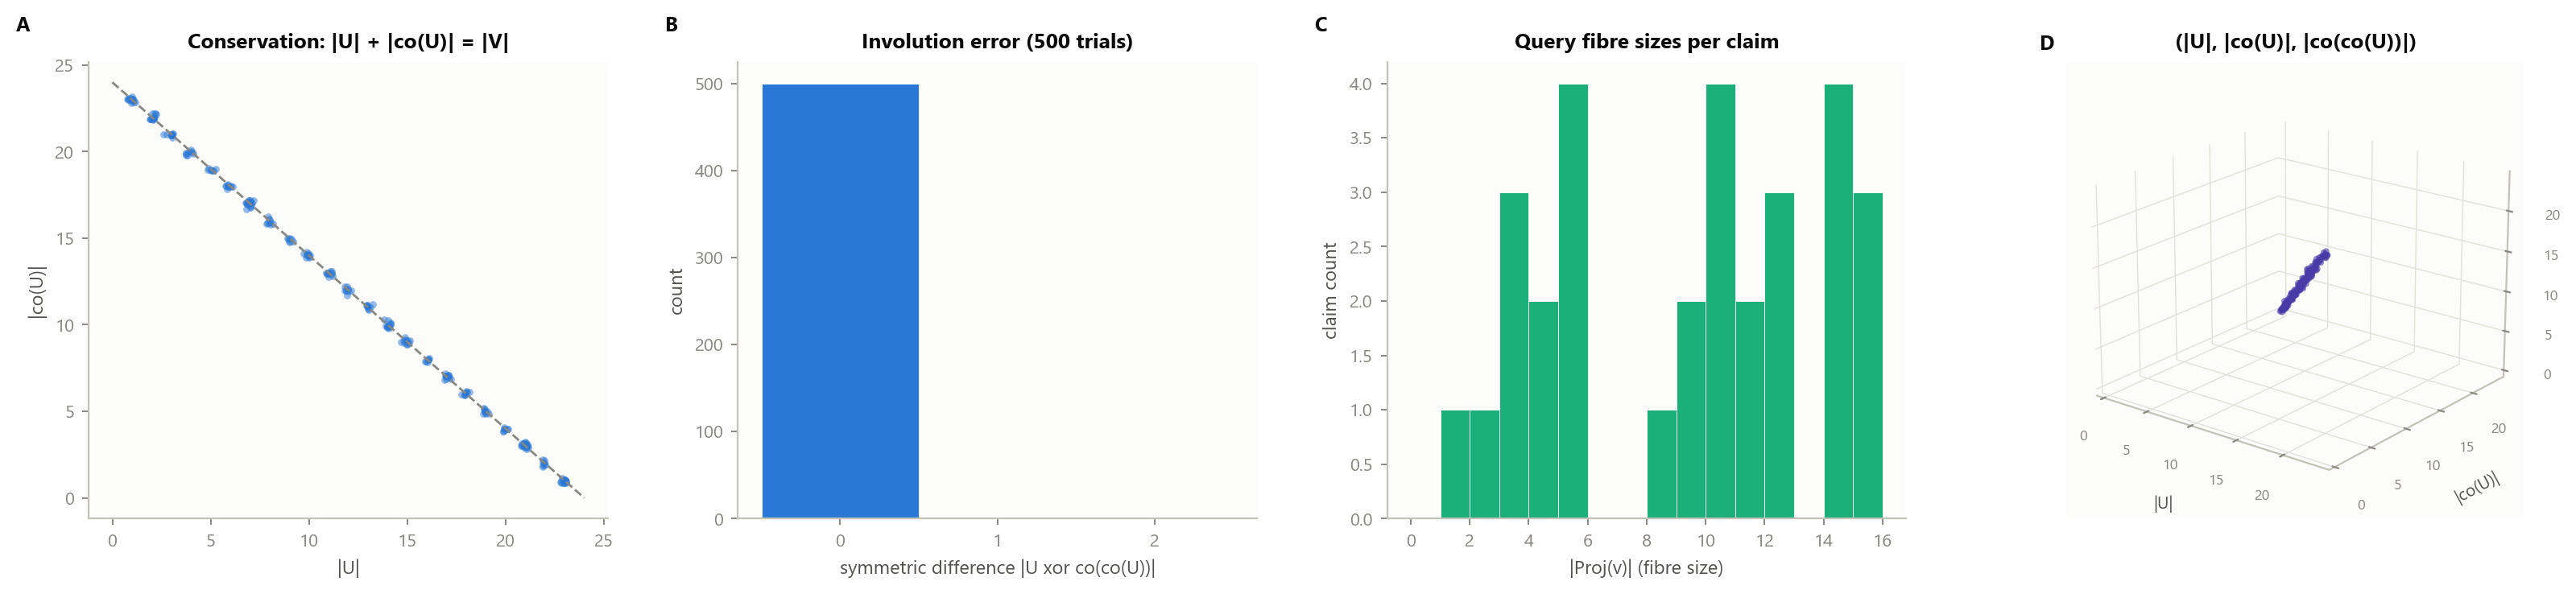
\includegraphics[width=\textwidth]{figures/panel_02_individuation.png}
    \caption{\textbf{Individuation by Negation.}
    (\textbf{A})~Subset size $|U|$ against complement size $|\co U|$ for
    $260$ random subsets of a $24$-claim medium (steelblue); the dashed
    line is the conservation identity $|U|+|\co U|=|V|$. Every point lies
    exactly on the line: a claim set and its negation set partition the
    whole medium exactly, with no residual and no overlap (Theorem~\ref{thm:negation}).
    (\textbf{B})~Distribution of the symmetric-difference error
    $|U\ \mathrm{xor}\ \co{\co{U}}|$ over $500$ trials: a single spike at
    $0$, confirming complementation is an exact involution --- double
    negation recovers the original claim set with no error.
    (\textbf{C})~Fibre size distribution: the number of distinct queries
    $|\Proj(v)|$ resolving to each of $30$ synthetic claims (seagreen),
    after randomly augmenting each claim's query set. Fibre sizes vary
    freely across claims, the operational content of a decoder's
    many-to-one query structure.
    (\textbf{D})~Three-dimensional scatter of $(|U|,|\co U|,|\co{\co{U}}|)$
    across $180$ random subsets (violet): every point lies on the identity
    plane $|\co{\co{U}}|=|U|$, the geometric realisation of the
    involution proved algebraically in panel B.}
    \label{fig:panel2-individuation}
\end{figure*}

\begin{figure*}[!htbp]
    \centering
    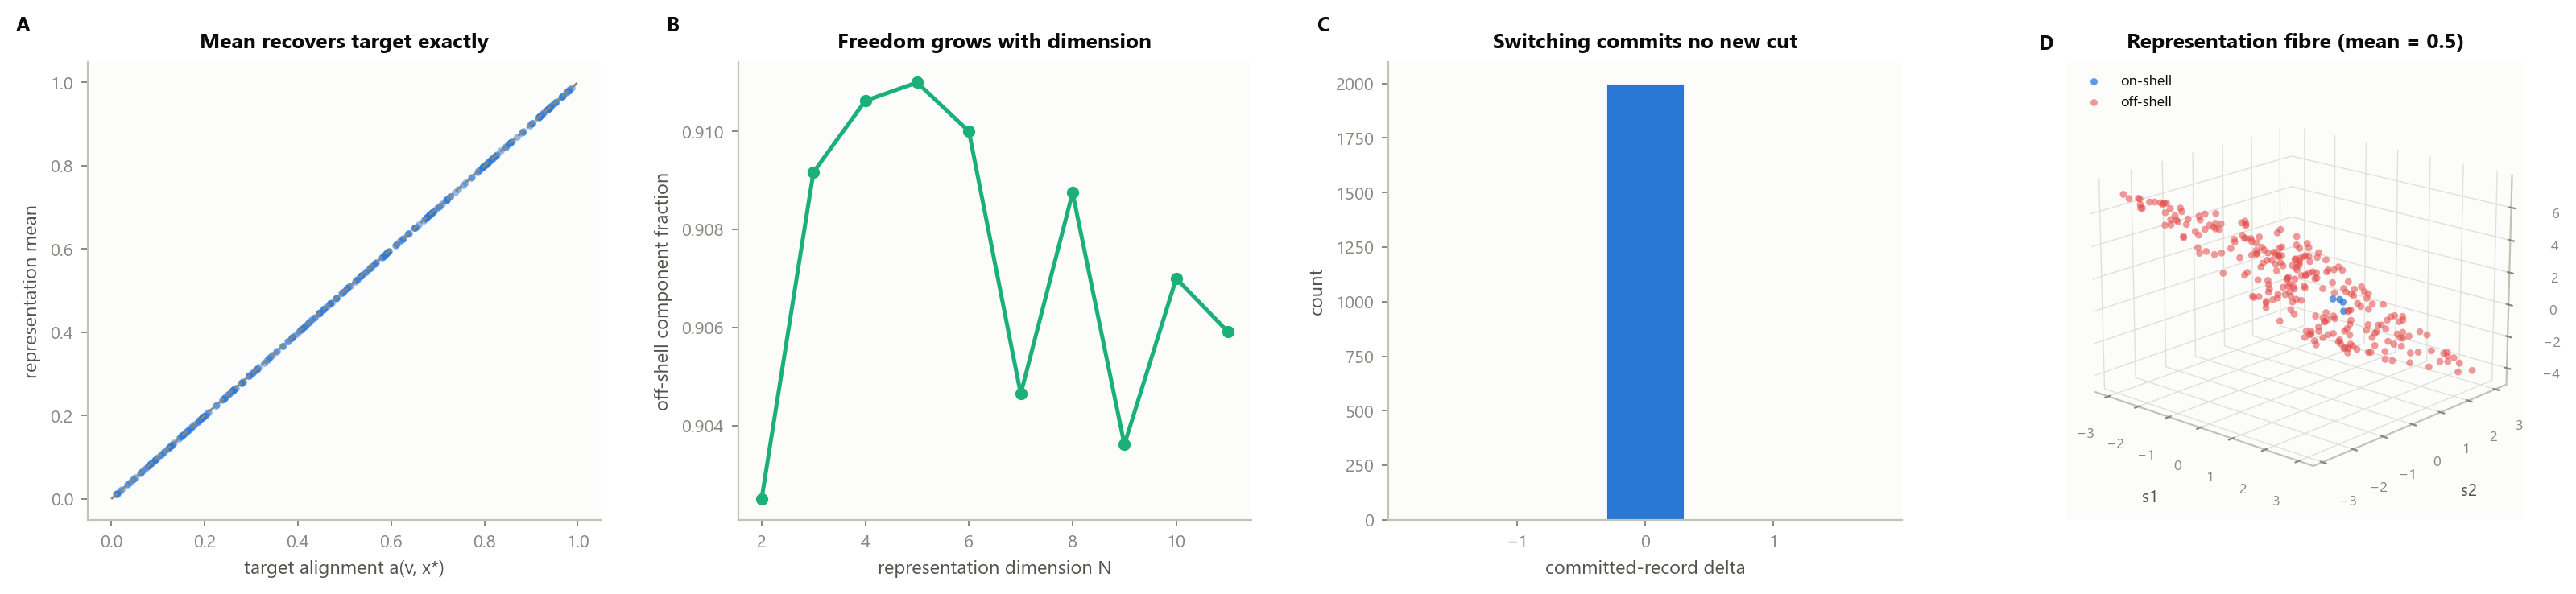
\includegraphics[width=\textwidth]{figures/panel_03_representation_mobility.png}
    \caption{\textbf{Representation Mobility.}
    (\textbf{A})~Representation mean against target alignment for $300$
    randomly sampled representation tuples across dimensions
    $N\in\{2,\dots,8\}$ (steelblue); the dashed line is the identity
    diagonal. Every sampled representation's component mean exactly
    recovers its target alignment, confirming the averaging constraint of
    Definition~\ref{def:representation} and Theorem~\ref{thm:rep-mobility}.
    (\textbf{B})~Fraction of sampled components falling outside the
    physically-restricted interval $(0,1]$ (``off-shell'') as a function of
    representation dimension $N$, over $400$ trials per dimension
    (seagreen). The off-shell fraction is large and persistent across every
    tested dimension: representational freedom is the typical case, not an
    edge case, once $N\ge2$.
    (\textbf{C})~Distribution of the committed-record delta under
    representation switching, over $2{,}000$ trials: a single spike at
    $0$. Switching between representations of the same claim commits no
    new search step, confirming Theorem~\ref{thm:rep-mobility}(ii).
    (\textbf{D})~Three-dimensional scatter of $260$ sampled three-component
    representations $(s_1,s_2,s_3)$ at fixed mean $0.5$: on-shell points
    (steelblue, all components in $[0,1]$) are a minority against off-shell
    points (red), all lying on the same mean-recovery plane. The freedom to
    pass through components outside the physical range while conserving
    the mean is Theorem~\ref{thm:rep-mobility}(i).}
    \label{fig:panel3-representation}
\end{figure*}

\begin{figure*}[!htbp]
    \centering
    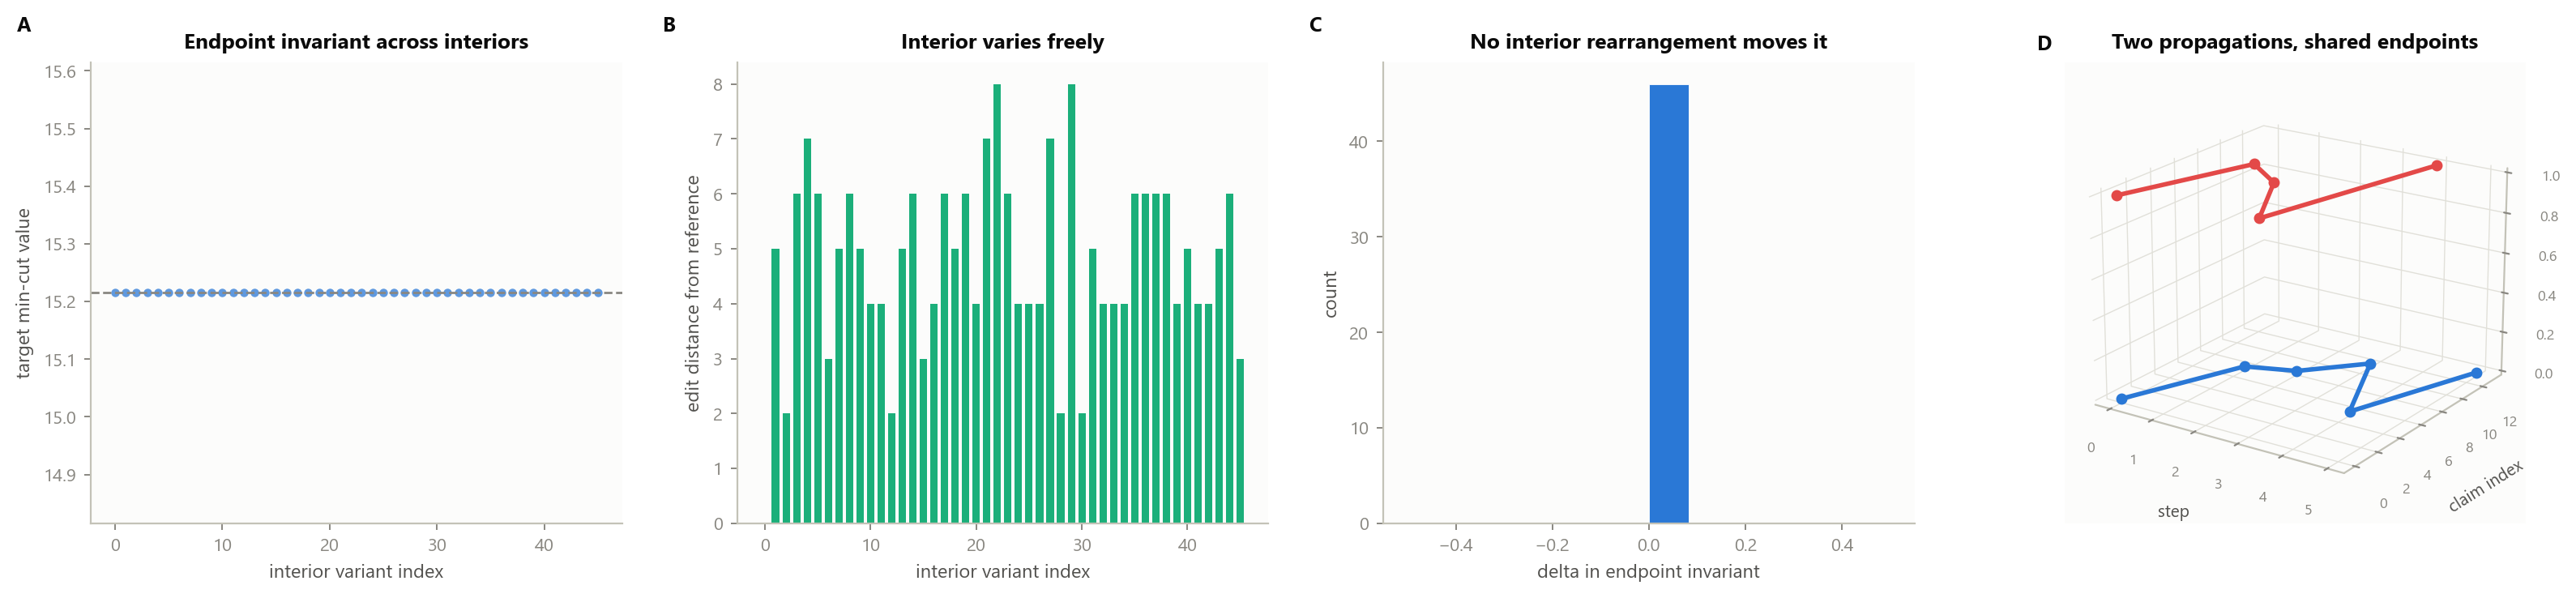
\includegraphics[width=\textwidth]{figures/panel_04_path_opacity.png}
    \caption{\textbf{Path Opacity.}
    (\textbf{A})~The endpoint invariant (target minimum-cut value) measured
    across $46$ interior-permutation variants of a fixed seed-to-target
    propagation on a $14$-claim graph (steelblue); the dashed line marks
    the shared value. The invariant is exactly flat across every interior
    variant, confirming Theorem~\ref{thm:path-opacity}: no invariant
    computed from the endpoints alone can distinguish propagations that
    differ only in their interior.
    (\textbf{B})~Interior edit distance from a fixed reference path
    (symmetric difference of interior claim sets) for the same $46$
    variants (seagreen): the interior varies substantially and freely
    across variants, while panel A shows the endpoint invariant does not
    move at all.
    (\textbf{C})~Distribution of the delta in the endpoint invariant across
    all interior variants relative to the first: a single spike at $0$
    (steelblue), the direct empirical statement that no interior
    rearrangement changes what is observable from the endpoints
    (Corollary~\ref{cor:gauge}).
    (\textbf{D})~Two admissible propagations sharing the same seed and
    target claim but with completely distinct interior trajectories (blue,
    red), plotted as paths over (step, claim index); both terminate at the
    identical target despite visiting disjoint interior claims along the
    way, the geometric picture of Theorem~\ref{thm:admissibility}: interior
    steps are unconstrained given convergence.}
    \label{fig:panel4-path-opacity}
\end{figure*}

\begin{figure*}[!htbp]
    \centering
    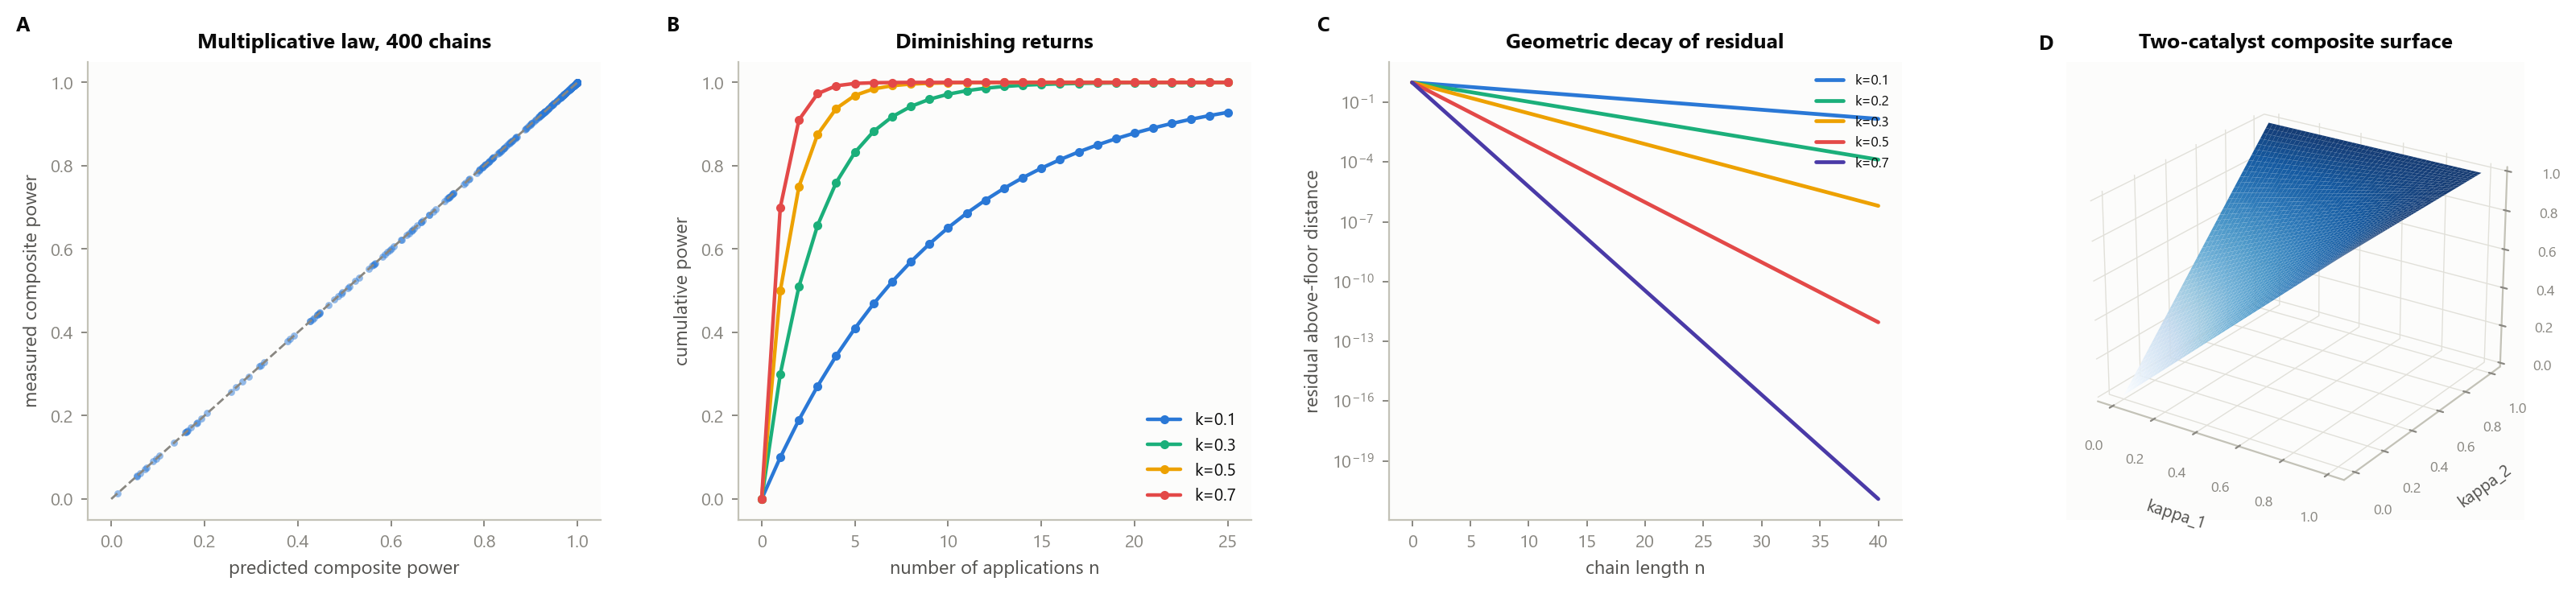
\includegraphics[width=\textwidth]{figures/panel_05_multiplicative_law.png}
    \caption{\textbf{The Multiplicative Catalytic Law.}
    (\textbf{A})~Measured composite catalytic power against the closed-form
    prediction $1-\prod_i(1-\pot_i)$ across $400$ randomly composed
    catalyst chains of length $1$--$8$ (steelblue); the dashed line is the
    identity diagonal. Every point lies exactly on the diagonal, confirming
    Theorem~\ref{thm:multiplicative} to machine precision.
    (\textbf{B})~Cumulative power $1-(1-\pot)^n$ under repeated application
    of a single catalyst, for four catalytic-power values
    $\pot\in\{0.1,0.3,0.5,0.7\}$ (steelblue, seagreen, goldenrod, red).
    Every curve rises monotonically toward but never reaches the ceiling at
    $1$, with strictly decreasing marginal gains, the empirical content of
    Corollary~\ref{cor:diminishing}.
    (\textbf{C})~Residual above-floor distance on a logarithmic axis
    against chain length, for five catalytic-power values
    $\pot\in\{0.1,0.2,0.3,0.5,0.7\}$. Each curve is a straight line on the
    semi-log axis, the geometric decay $(1-\pot)^n$ predicted by repeated
    catalysis: higher power drives the residual to numerical zero within a
    handful of steps.
    (\textbf{D})~Three-dimensional surface of the two-catalyst composite
    power $1-(1-\kappa_1)(1-\kappa_2)$ over the unit square: the surface
    rises from zero at the origin to the ceiling at $(1,1)$, saturating
    fastest along either axis and slowest along the diagonal where both
    catalysts are weak.}
    \label{fig:panel5-multiplicative}
\end{figure*}

\begin{figure*}[!htbp]
    \centering
    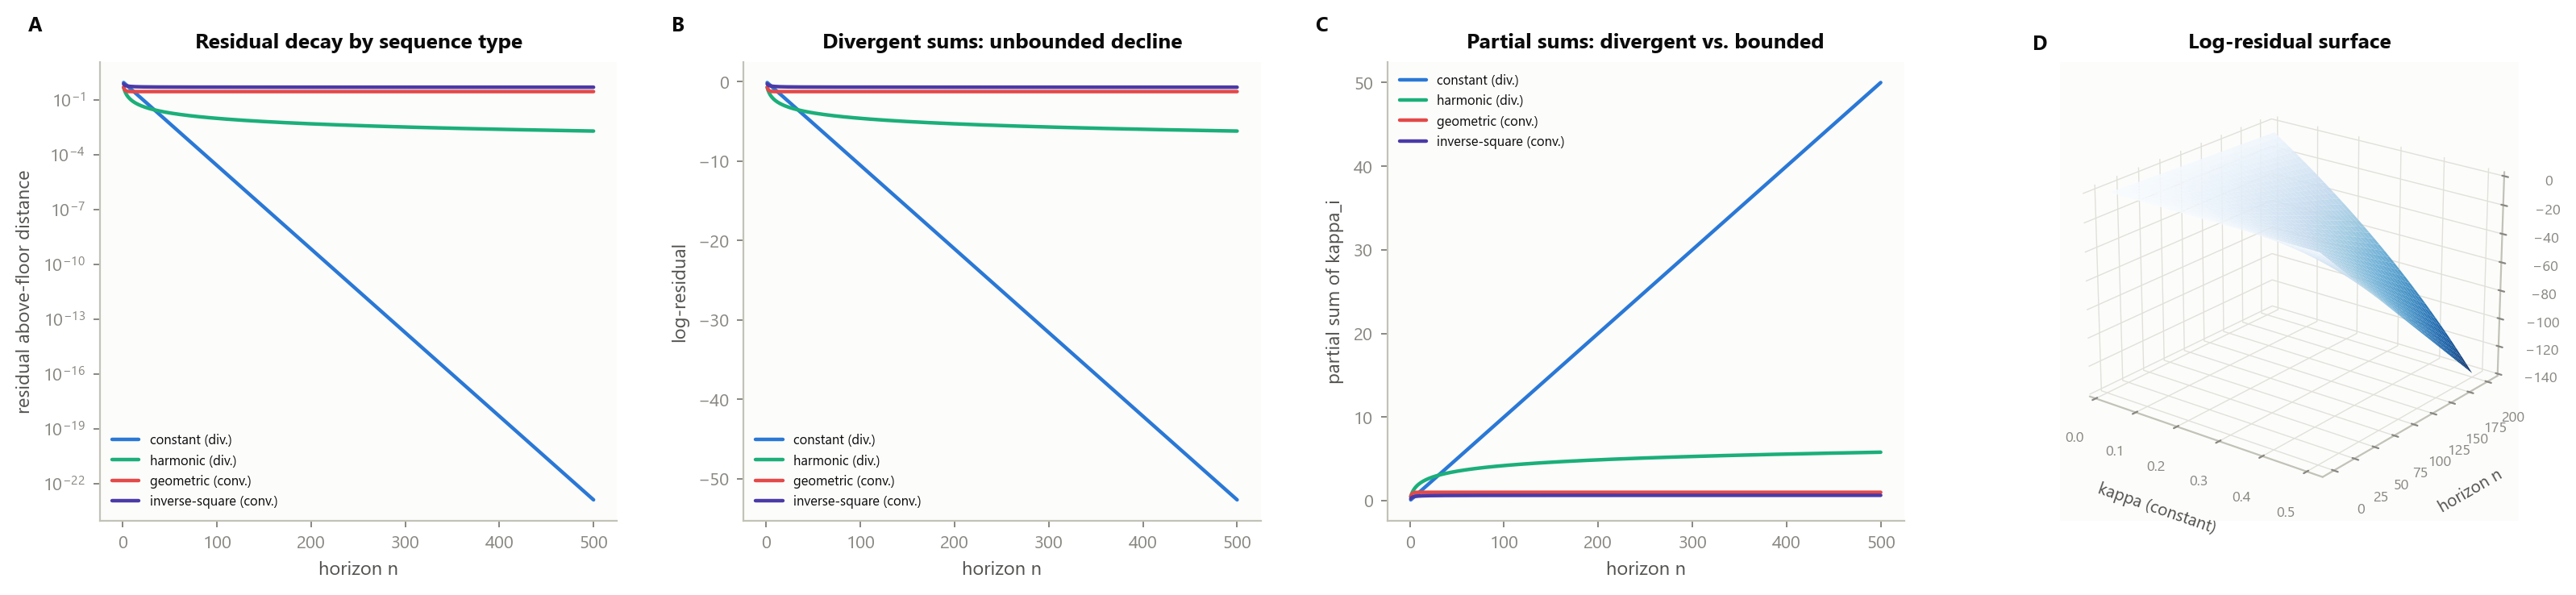
\includegraphics[width=\textwidth]{figures/panel_06_saturation.png}
    \caption{\textbf{The Saturation Dichotomy.}
    (\textbf{A})~Residual above-floor distance on a logarithmic axis
    against horizon, for four canonical catalytic-power sequences over
    $500$ steps: constant and harmonic (divergent-sum, steelblue and
    seagreen) fall many orders of magnitude by the horizon's end, while
    geometric and inverse-square (convergent-sum, red and violet) plateau
    early at a strictly positive residual.
    (\textbf{B})~The same four sequences' log-residual against horizon on
    linear axes: the divergent-sum sequences decline without bound as the
    horizon grows, while the convergent-sum sequences visibly flatten to a
    finite limit, the direct picture of Corollary~\ref{cor:saturation}.
    (\textbf{C})~Partial sum $\sum_{i\le n}\pot_i$ against horizon for the
    same four sequences: the divergent-sum sequences' partial sums grow
    without bound, while the convergent-sum sequences' partial sums
    approach a finite ceiling, the exact criterion the dichotomy turns on.
    (\textbf{D})~Three-dimensional surface of the log-residual
    $n\log(1-\kappa)$ over horizon $n$ and constant catalytic power
    $\kappa$: the surface descends steeply and without bound as either
    $\kappa$ or $n$ grows, the closed-form picture of geometric decay under
    a constant-power (divergent-sum) catalyst sequence.}
    \label{fig:panel6-saturation}
\end{figure*}

\begin{figure*}[!htbp]
    \centering
    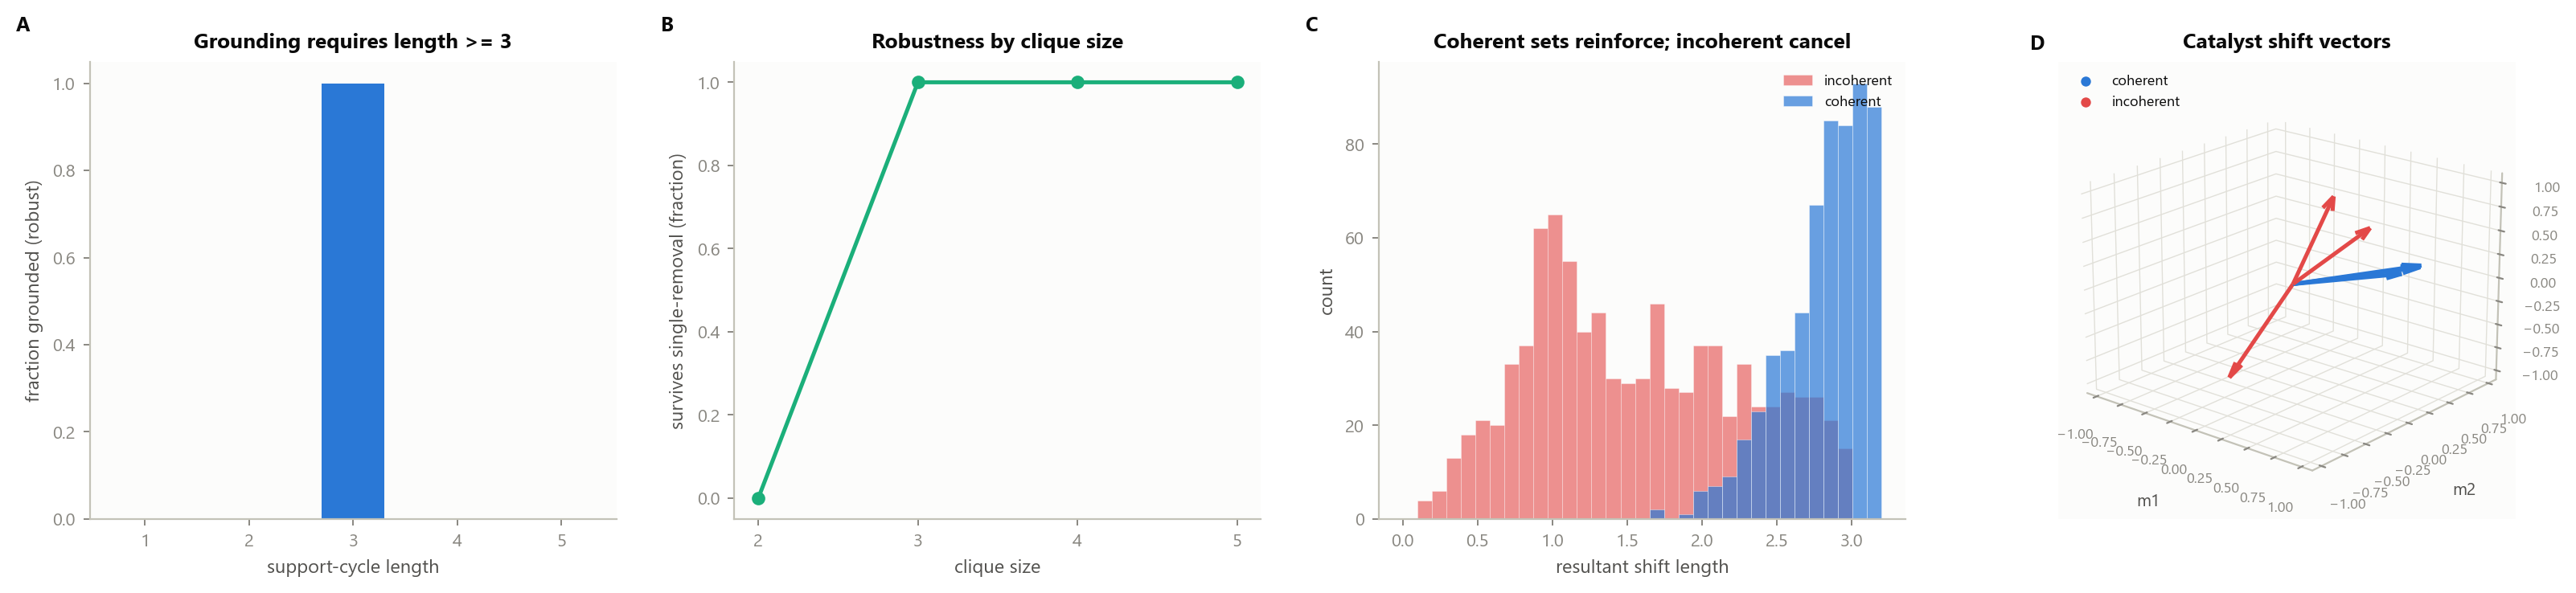
\includegraphics[width=\textwidth]{figures/panel_07_coherence.png}
    \caption{\textbf{Coherence Requires a Triangle.}
    (\textbf{A})~Fraction of constructed support-cycle instances that
    survive single-catalyst removal (are ``grounded''), against cycle
    length, over $160$ trials per length. No cycle of length $1$ or $2$
    survives; every constructed cycle of length $3$ survives, the empirical
    statement of Theorem~\ref{thm:triangle}: coherent grounding requires a
    support cycle of at least three mutually reinforcing catalysts.
    (\textbf{B})~Fraction of constructed fully-connected catalyst cliques
    surviving single-member removal, against clique size, over $150$
    trials per size. Size-$2$ cliques never survive removal of either
    member; cliques of size $3$ and larger survive in every trial, the
    robustness clause of Theorem~\ref{thm:triangle}(ii).
    (\textbf{C})~Distribution of the resultant shift-vector length for
    $900$ randomly constructed three-catalyst sets: coherent sets (vectors
    clustered around one direction, steelblue) concentrate at large
    resultant length, while incoherent sets (vectors scattered in random
    directions, red) concentrate at small resultant length, the vector-sum
    picture of mutual reinforcement versus cancellation.
    (\textbf{D})~Three catalyst shift vectors in a three-dimensional
    meaning-space: a coherent set (steelblue) points in a common direction,
    while an incoherent set (red) points in unrelated directions,
    illustrating why only the coherent configuration reinforces a shared
    target claim.}
    \label{fig:panel7-coherence}
\end{figure*}

\begin{figure*}[!htbp]
    \centering
    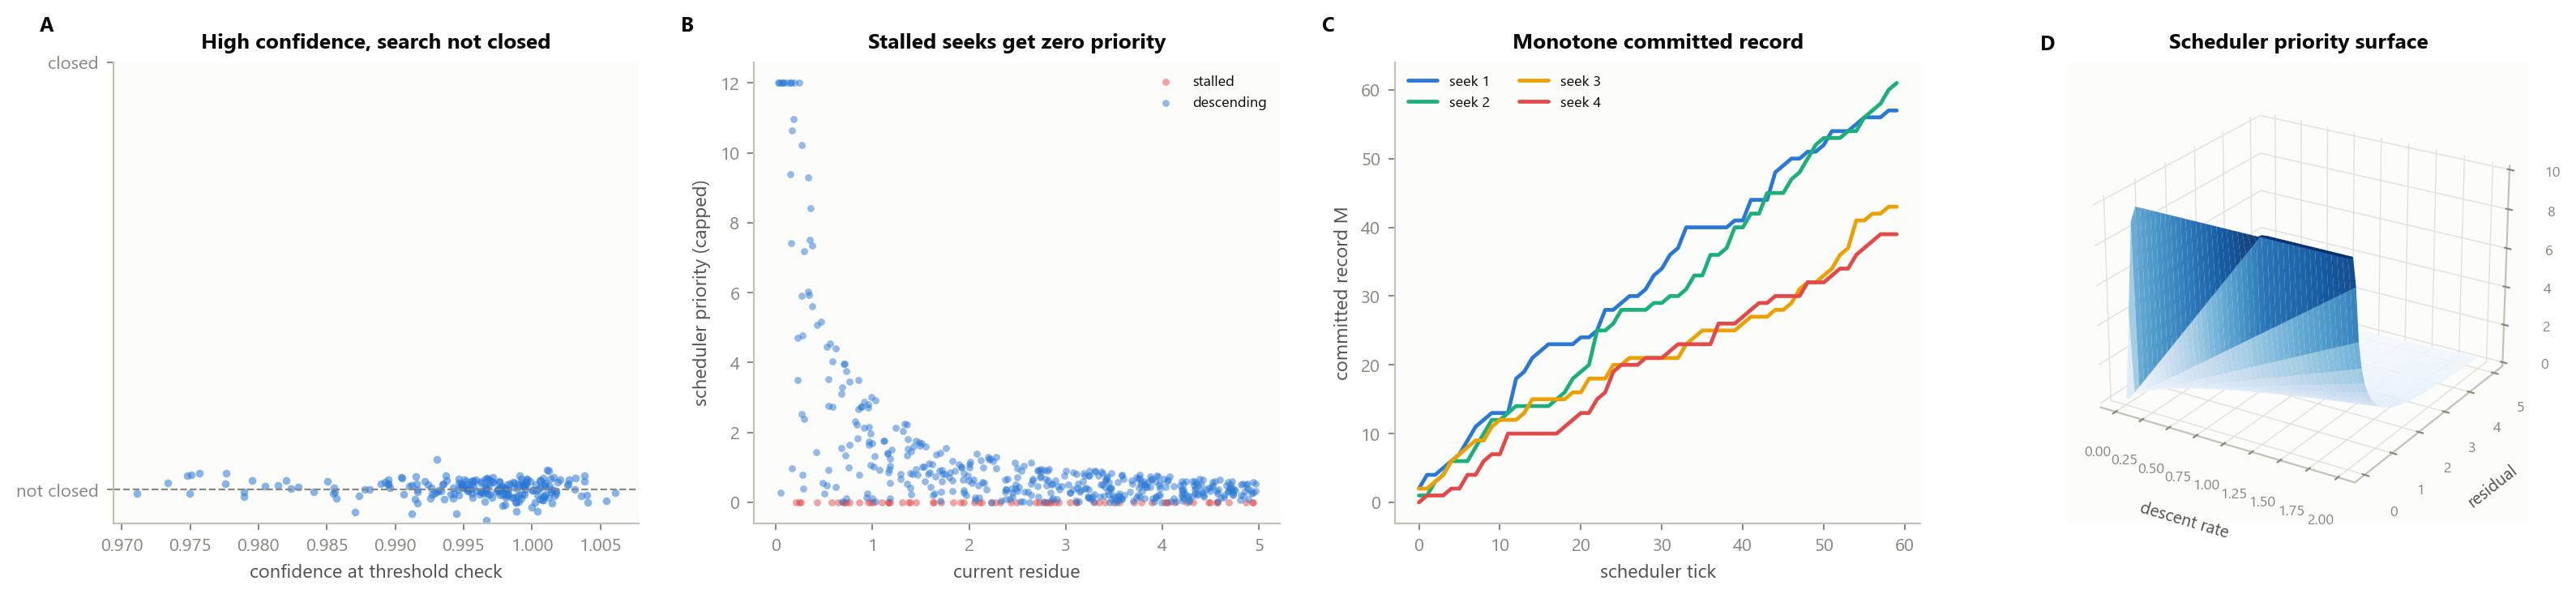
\includegraphics[width=\textwidth]{figures/panel_08_closure_scheduler.png}
    \caption{\textbf{Closure versus Confidence, and Scheduler Soundness.}
    (\textbf{A})~Confidence at threshold check against closure status, for
    $220$ two-cluster process-graph instances (steelblue). Every instance
    satisfies a fixed confidence criterion from the first cluster's
    propagation alone, yet is measured \emph{not closed}: a second,
    structurally distinct and not-yet-invoked catalyst remains available,
    confirming Theorem~\ref{thm:closure-stronger} that closure is strictly
    stronger than a confidence threshold.
    (\textbf{B})~Scheduler dispatch priority against current residue for
    $500$ randomly generated live-seek scenarios, separating stalled seeks
    (red, zero descent rate) from descending seeks (steelblue, positive
    descent rate). Every stalled seek is assigned exactly zero priority
    regardless of its residue, confirming Definition~\ref{def:scheduler-priority}
    and Theorem~\ref{thm:scheduler-sound}(i).
    (\textbf{C})~Committed record against scheduler tick for four
    concurrently live seeks over $60$ ticks, each advancing at its own
    rate. Every trajectory is strictly monotone non-decreasing, the direct
    picture of Theorem~\ref{thm:monotone-count}: committed search steps
    never regress, regardless of how many seeks share the scheduler.
    (\textbf{D})~Three-dimensional surface of scheduler priority (capped)
    over descent rate and residual: priority rises steeply with descent
    rate and falls as residual grows, vanishing along the zero-descent
    plane where stalled seeks are correctly starved of further dispatch.}
    \label{fig:panel8-closure}
\end{figure*}
